\appendixitem{定义}

定义 1. 组合图（或在不会引起混淆时简称为图）是一对 \((\mathrm{A},\mathrm{S})\)，其中 \(\mathrm{S}\) 是一个集合，而 \(\mathrm{A}\) 是 \(\mathfrak{P}(\mathrm{S})\) 的一个子集，由具有两个元素的集合组成。

设 \(\Gamma = (A, S)\) 是一张图。A 中的元素称为边，S 中的元素称为 \(\Gamma\) 的顶点；如果 \(\{x, y\}\) 是一条边，则称两个顶点相连。如果一个顶点至多与一个顶点相连，则称其为端点；如果它至少与三个顶点相连，则称其为分叉点。

按照一般定义（集合论 R. §8），从图 \(\Gamma\) 到图 \(\Gamma' = (A', S')\) 的同构，是从 \(S\) 到 \(S'\) 的双射，将 \(A\) 映到 \(A'\)。图 \(\Gamma' = (A', S')\) 是 \(\Gamma\) 的子图，若 \(S' \subset S\) 且 \(A' \subset A\)；称 \(\Gamma\) 为 \(\Gamma\) 的满子图，若 \(S' \subset S\) 且 \(A' = A \cap \mathfrak{P}(S)\)。显然，\(S\) 的每个子集恰好是 \(\Gamma\) 的一个满子图的顶点集合。

为了使论证更易于理解，我们用一幅图表示一个图：图中有与顶点对应的点；当且仅当它们所表示的顶点在图中相连时，两个点由一条线相连。例如，图

\pandocbounded{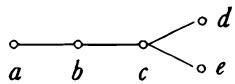
\includegraphics[keepaspectratio]{images/part001_959a1795.jpg}}

它表示一个图，其顶点为 \(a, b, c, d, e\)，其边为 \(\{a, b\}\)、\(\{b, c\}\)、\(\{c, d\}\) 和 \(\{c, e\}\)。

